\section{Durchf\"uhrung}
\label{sec:Durchfuehrung}
Im Folgenden werden alle Bezeichnungen der Quantenzustände gemäß der Konvention gewählt.
Für die Bahndrehimpulsquantenzahl $l$ sind aus historischem Grunde die Bezeichungen 
sharp (S),
principal (P),
diffuse (D),
fundamental (F).

Die Quantenzahlen $n,l,j$ werden in der Form $\mathup{nl}_\mathup{j}$, beispielsweise $3D_{\sfrac{5}{2}}$ angegeben.
\subsection{Aufbau des Gitterspektralapparates}
\begin{figure}
	\centering
	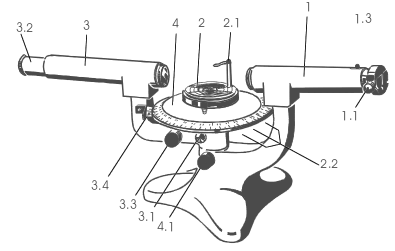
\includegraphics[width=0.7\textwidth]{Bilder/Apparat.png}
	\caption{Perspektivische Darstellung des verwendeten Gerätes. \cite{skript}} 
	\label{fig:Gitterspektralapparat}
\end{figure}
Der Gitterspektralapparat ist in Abbildung \ref{fig:Gitterspektralapparat} schematisch dargestellt.
Er besteht im Wesentlichen aus den drei Bestandteilen Kollimatorrohr, Gittertisch und Fernrohr.
An der Eintrittstelle des Kollimatorrohres befindet sich eine Spaltblende, durch welche das untersuchte Licht eintritt.
Auf der anderen Seite des Kollimatorrohres befindet sich ein Gittertisch mit Gitter, welche im Gegensatz zum Kollimatorohr beweglich sind und sich somit um eine vertikale Achse drehen lässt. 
Im System kommen Linsen zum Einsatz, damit das im Allgemeinen divergente Licht von der Probe parallel eintritt und auf das Gitter trifft.
%Spaltblende und Linse am Kollimatorrohr sorgen für kohärentes Licht.
Das Fernrohr ist zur die Beobachtung des vom Gitter abgelenkten Lichtes geeignet und kann unabhängig vom Gittertisch gedreht und fein eingestellt werden. 
Es erfügt darüber hinaus über eine Linse, die das Licht von dem Gitter auf eine Brennebene fokussiert, und ein Fadenkreuz.
Somit kann ein reelles Bild des Gitters mit dem Fadenkreuz ausgewertet werden.

Für die Justierung müssen Spalt und Fadenkreuz jeweils in den Brennebenen der zugehörigen Objektive sein, die Gitteröffnung vertikal, die Spaltblende kleinstmöglich und die Gitterebene senkrecht zum einfallenden Strahl sein. 
Es wird ein scharfes Beugungsbild sichtbar.
Nach der Justierung wird der Gittertisch festgesetzt und als unbeweglich angesehen.
%Zur Probe kann das Beugungsbild des Gitters beobachtet werden, es sollte sich beim Durchschwenken des Fernrohres keine vertikale Bewegung des Bildes zeigen.
Zur Bestimmung von $\mathup{\Delta}\lambda$ wird das Okularmikrometer benützt.
Es wird anhand des Mikrometers der Abstand der Dublettlinien in Skaleneinheiten ausgemessen, hierzu ist eine Eichung notwenig.
Dies geschieht durch die Wahl zweier Spektrallinien, deren Wellenlänge bekannt sind und die gleichzeitig durch das Fernrohr beobachtbar sind.
Der gemessene Abstand $\mathup{\Delta}s$ von Dublett-Linien lässt sich mithilfe der Formel
\begin{equation}
	\mathup{\Delta}\lambda=\frac{\cos{\bar\phi}}{\cos{\bar\phi_{1,2}}}\frac{\mathup{\Delta}s}{\mathup{\Delta}t}(\lambda_1-\lambda_1)
\end{equation}
umrechnen, in welcher $\bar\phi_{1,2}$ der gemittelte Wert zwischen zwei Spektrallinien, $\bar\phi$ der gemittelte Wert zwischen den Dublett-Linien, $\mathup{\Delta}s$ der Abstand der Dublett-Linien und $\mathup{\Delta}t$ der Abstand zweier Spektrallinien ist.

\subsection{Messprogramm}
Zur Kalibrierung der Apparatur werden die Beugungswinkel der Spektrallinien von Helium gemessen.
Die Wellenlängen sind in Tabelle \ref{tab:hgspektrum} angegeben.
Anschließend wird das Okularmikrometer mit den grünen oder violetten Spektrallinien skaliert und somit die Messung an Alkali-Atomen ermöglicht.

Es werden Natrium-, Kalium- und Rubidium-Spektren betrachtet.
Im Einzelnen werden die Linien der Farben
\begin{itemize}
	\item{Natrium:\hspace{10pt}rot, gelb, grüngelb}
	\item{Kalium:\hspace{15pt}zweimal gelb, zweimal grün}
	\item{Rubidium:\hspace{3pt}rot (3. und 4. Linie)}
\end{itemize}
genau untersucht, hier wird mithilfe des Okularmikrometers die Distanz der Dublett-Strukturen bestimmt.
Abschließend wird das Auflösevermögen bestimmt, indem die Breite des Spaltes in der Nähe des Gitter so klein gewählt wird, dass die Spektrallinien verschmelzen.
Dies wird am gelben Natrium-Dublett durchgeführt.